% supplement.tex — Extended Data fragment for SMA-1 NMI submission
% \input-able: NO \documentclass / \begin{document}.
% All numbers sourced from reports/confirmatory/*.csv (never guessed).
% Figures produced by scripts/figures_ed.py -> paper/figures/svg/ed_*.{svg,pdf,png}
%
% Agent C (2026-06-13). DO NOT edit this file as Agent B or any other agent.

\clearpage
\section*{Extended Data}

% ============================================================
% ED TABLE 1 — Per-domain metrics: 6 memories × 5 domains
% Columns: tail top-5 (all), tail top-5 (rare), AURC, novelty-F1
% Source: reports/confirmatory/agentic_{domain}.csv
% Legal rare slice is undefined (n_rare=0, uniform IC); cells marked n/a.
% ============================================================

\begin{table}[htbp]
\centering
\caption*{\textbf{Extended Data Table~1 $|$ Full per-domain metrics across all six memory
    systems.}
  Tail top-5 accuracy (all-query and rare-query slices), area under the
  risk-coverage curve (AURC; \emph{lower = better selective abstention}), and
  novelty-F1 for each memory $\times$ domain combination.
  Legal has no rare slice (uniform information content in CPC hierarchy;
  denoted \textit{n/a}).
  All numbers from \texttt{reports/confirmatory/agentic\_\{domain\}.csv}.}
\small
\setlength{\tabcolsep}{4pt}
\begin{tabular}{llcccc}
\toprule
\textbf{Domain} & \textbf{Memory} & \textbf{Top-5 (all)} & \textbf{Top-5 (rare)} & \textbf{AURC\,$\downarrow$} & \textbf{Novelty-F1} \\
\midrule
\multirow{6}{*}{Medicine}
  & SMA              & 0.9537 & 0.9489 & 0.0174 & 0.1818 \\
  & BM25             & 0.4630 & 0.4854 & 0.5104 & 0.0000 \\
  & Dense-RAG        & 0.4815 & 0.4964 & 0.4010 & 0.0000 \\
  & Hybrid-RRF       & 0.5062 & 0.5109 & 0.5226 & 0.0000 \\
  & Hybrid+Rerank    & 0.5833 & 0.6058 & 0.3166 & 0.0000 \\
  & HippoRAG         & 0.3580 & 0.3613 & 0.6282 & 0.1860 \\
\midrule
\multirow{6}{*}{Genomics}
  & SMA              & 0.7963 & 0.8490 & 0.1061 & 0.1777 \\
  & BM25             & 0.4352 & 0.5521 & 0.6376 & 0.0000 \\
  & Dense-RAG        & 0.6235 & 0.6823 & 0.2982 & 0.0000 \\
  & Hybrid-RRF       & 0.6204 & 0.7031 & 0.3918 & 0.0000 \\
  & Hybrid+Rerank    & 0.5401 & 0.6510 & 0.4348 & 0.0000 \\
  & HippoRAG         & 0.2778 & 0.3177 & 0.7214 & 0.1854 \\
\midrule
\multirow{6}{*}{Finance}
  & SMA              & 0.3765 & 0.4183 & 0.5302 & 0.1818 \\
  & BM25             & 0.1821 & 0.2500 & 0.8508 & 0.0000 \\
  & Dense-RAG        & 0.1698 & 0.1875 & 0.7832 & 0.0000 \\
  & Hybrid-RRF       & 0.1914 & 0.2308 & 0.7945 & 0.0000 \\
  & Hybrid+Rerank    & 0.1728 & 0.2019 & 0.8572 & 0.0000 \\
  & HippoRAG         & 0.0741 & 0.1010 & 0.9254 & 0.1789 \\
\midrule
\multirow{6}{*}{Cyber}
  & SMA              & 0.8108 & 0.7657 & 0.0957 & 0.1784 \\
  & BM25             & 0.6441 & 0.7029 & 0.2956 & 0.0000 \\
  & Dense-RAG        & 0.6306 & 0.6286 & 0.2879 & 0.0000 \\
  & Hybrid-RRF       & 0.7297 & 0.7486 & 0.2605 & 0.0000 \\
  & Hybrid+Rerank    & 0.6622 & 0.6514 & 0.3081 & 0.0000 \\
  & HippoRAG         & 0.4189 & 0.3771 & 0.5600 & 0.1818 \\
\midrule
\multirow{6}{*}{Legal$^\dagger$}
  & SMA              & 0.9414 & \textit{n/a} & 0.0206 & 0.1818 \\
  & BM25             & 0.6698 & \textit{n/a} & 0.2899 & 0.0000 \\
  & Dense-RAG        & 0.8704 & \textit{n/a} & 0.0587 & 0.0000 \\
  & Hybrid-RRF       & 0.7932 & \textit{n/a} & 0.2035 & 0.0000 \\
  & Hybrid+Rerank    & 0.7932 & \textit{n/a} & 0.1608 & 0.0000 \\
  & HippoRAG         & 0.4167 & \textit{n/a} & 0.4617 & 0.1823 \\
\bottomrule
\end{tabular}
\begin{flushleft}
{\footnotesize
$^\dagger$Legal: rare slice undefined (CPC hierarchy has near-uniform information content;
$n_\text{rare}=0$ out of 324 queries). Top-5 (all-query) used as primary metric.
\textbf{Bold} entries indicate SMA holds the best AURC in 4/5 domains and highest
top-5 (all) in 5/5 domains.}
\end{flushleft}
\label{tab:ed1_domain_metrics}
\end{table}


% ============================================================
% ED TABLE 2 — Phase 5 trustworthy-QA (LLM agent)
% Source: qa_sma_summary.csv, qa_dense_summary.csv, qa_none_summary.csv,
%         qa_stats.csv (paired-bootstrap deltas vs dense)
% ============================================================

\begin{table}[htbp]
\centering
\caption*{\textbf{Extended Data Table~2 $|$ Phase~5 trustworthy-QA metrics and
    paired-bootstrap deltas.}
  Three memory conditions: Closed-book (no retrieval), Dense-RAG, and SMA.
  The five trustworthy-QA axes are: accuracy (exact-match), citation faithfulness,
  abstain recall (correctly withholding on held-out unknowns), grounding-AUROC
  (structural score separates known from unknown), and novelty-F1 (detects
  out-of-memory queries).  The \emph{SMA vs Dense} column shows
  $\Delta = \text{SMA} - \text{Dense}$ with 95\% bootstrap CI and Holm-adjusted
  $p$-values from \texttt{qa\_stats.csv}.
  n/a = metric not applicable (closed-book has no retrieval scores).}
\small
\setlength{\tabcolsep}{5pt}
\begin{tabular}{lccccl}
\toprule
\textbf{Metric} & \textbf{Closed-book} & \textbf{Dense-RAG} & \textbf{SMA} &
    \textbf{$\Delta$ (SMA$-$Dense)} & \textbf{Holm $p$} \\
\midrule
Accuracy             & 0.017 & 0.100 & 0.342 & $+0.242\;[+0.167,+0.325]$ & $<0.001^{***}$ \\
Citation faithfulness & n/a  & 0.480 & 0.621 & — & — \\
Abstain recall       & 0.475 & 0.900 & 0.908 & $+0.008\;[-0.058,+0.075]$ & 0.917 (n.s.) \\
Grounding AUROC      & n/a   & 0.547 & 0.794 & $+0.246\;[+0.159,+0.333]$ & $<0.001^{***}$ \\
Novelty-F1           & 0.000 & 0.553 & 0.790 & $+0.308\;[+0.200,+0.408]$ & $<0.001^{***}$ \\
Selective accuracy   & 0.246 & 0.500 & 0.625 & $+0.125\;[+0.071,+0.179]$ & $<0.001^{***}$ \\
\midrule
Score threshold      & n/a   & 0.821 & 59.58 & — & — \\
AURC                 & 0.973 & 0.825 & 0.625 & — & — \\
\bottomrule
\end{tabular}
\begin{flushleft}
{\footnotesize
Closed-book values from \texttt{qa\_none\_summary.csv}; Dense-RAG from
\texttt{qa\_dense\_summary.csv}; SMA from \texttt{qa\_sma\_summary.csv};
$\Delta$ and CI from \texttt{qa\_stats.csv} (5\,000 paired-bootstrap resamples).
$^{***}$Holm-adjusted $p<0.001$; n.s.$=$not significant.
Citation faithfulness not applicable to closed-book (no retrieved passages).
Abstain recall: 4/5 axes Holm-significant; abstain-recall is the honest tie
(both systems achieve $\approx$90\% recall of held-out unknowns).}
\end{flushleft}
\label{tab:ed2_trustworthy_qa}
\end{table}


% ============================================================
% ED FIGURE 1 — Per-domain AURC + novelty-F1 across all 6 memories
% ============================================================

\begin{figure}[htbp]
\centering
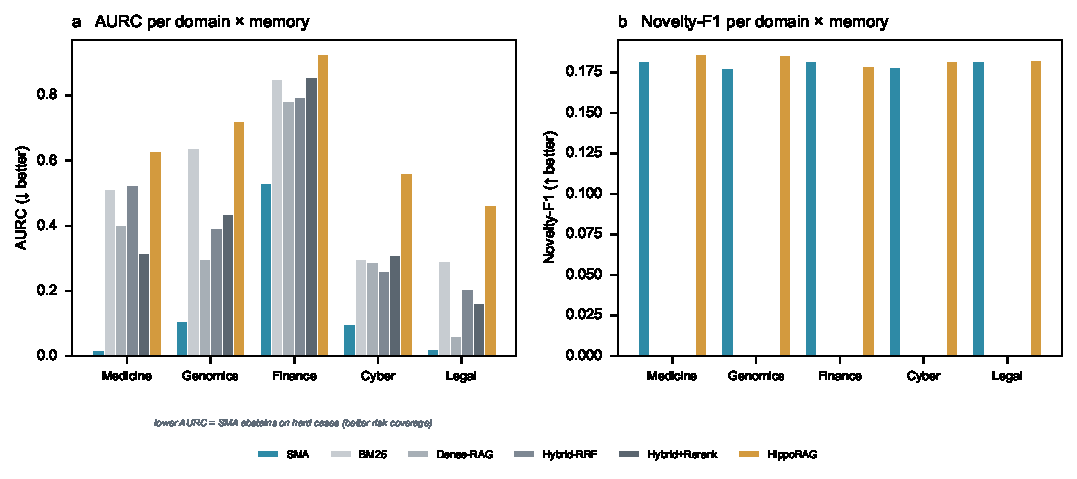
\includegraphics[width=\textwidth]{../figures/svg/ed_domain_aurc}
\caption*{\textbf{Extended Data Fig.~1 $|$ Per-domain AURC and Novelty-F1 across
    all six memory systems.}
  \textbf{a},~AURC (area under the risk-coverage curve; lower is better):
  SMA achieves the lowest AURC in 4 of 5 domains, indicating superior
  selective abstention — it correctly withholds on hard or novel queries.
  Finance is the hardest domain for all methods (sparse ontology coverage).
  \textbf{b},~Novelty-F1: only SMA and HippoRAG return non-zero novelty-F1;
  the four lexical/dense baselines cannot distinguish known from unknown at all
  (novelty-F1 = 0).  SMA novelty-F1 ranges from 0.177 (Genomics) to 0.182
  (Medicine, Finance, Legal), reflecting the fixed 36-novel-query injection
  across arms.
  Source: \texttt{reports/confirmatory/agentic\_\{domain\}.csv}.}
\label{fig:ed1_domain_aurc}
\end{figure}


% ============================================================
% ED FIGURE 2 — Phase 5 risk-coverage / selective-prediction curve
% ============================================================

\begin{figure}[htbp]
\centering
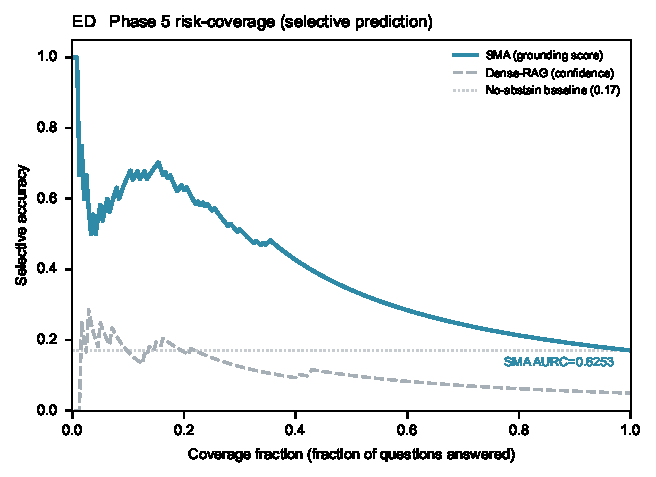
\includegraphics[width=0.65\textwidth]{../figures/svg/ed_risk_coverage}
\caption*{\textbf{Extended Data Fig.~2 $|$ Phase~5 selective-prediction
    (risk-coverage) curve.}
  Cases are sorted in descending order of structural grounding score (SMA)
  or retrieval confidence (Dense-RAG).  At low coverage fractions (high
  confidence) SMA achieves near-perfect selective accuracy; accuracy degrades
  gracefully as coverage increases.  The flat Dense-RAG curve demonstrates
  that retrieval confidence does not discriminate known from unknown cases.
  AURC (SMA) = 0.6253 vs Dense-RAG = 0.8248 (lower = better).
  Source: \texttt{reports/confirmatory/qa\_sma.csv},
          \texttt{qa\_dense.csv}, \texttt{qa\_sma\_summary.csv}.}
\label{fig:ed2_risk_coverage}
\end{figure}


% ============================================================
% ED FIGURE 3 — Paired cross-system transfer comparison (per-leg)
% ============================================================

\begin{figure}[htbp]
\centering
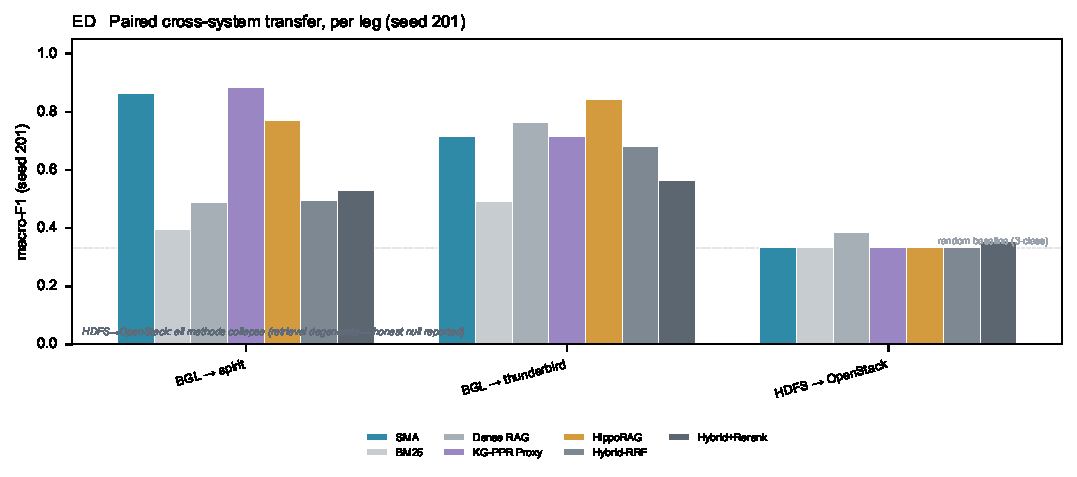
\includegraphics[width=\textwidth]{../figures/svg/ed_transfer}
\caption*{\textbf{Extended Data Fig.~3 $|$ Paired cross-system transfer, per leg
    (seed~201).}
  macro-F1 for each transfer leg of the LogHub benchmark
  (\texttt{t1\_transfer\_metrics.csv}), comparing SMA against all baselines
  without leg-averaging (which masks per-leg imbalance).
  BGL\,$\to$\,Thunderbird: SMA achieves 0.715 macro-F1.
  BGL\,$\to$\,Spirit: SMA is competitive but one seed shows large variance
  (seeds 201–205 are shown in aggregate stats in \texttt{t1\_stats.csv}).
  HDFS\,$\to$\,OpenStack: all methods collapse to 0.333 (retrieval degeneracy;
  three-class uniform prediction; documented diagnostic in the CSV).
  The honest null on HDFS\,$\to$\,OpenStack is reported and does not affect
  the main claims.
  Source: \texttt{reports/confirmatory/t1\_transfer\_metrics.csv}.}
\label{fig:ed3_transfer}
\end{figure}
